\documentclass[12pt,a4paper]{ctexart}  % 选择文档类型
% \usepackage{latexsym}
\usepackage{amsmath}   % aligned必须需要该宏宝
\usepackage[colorlinks,linkcolor=red]{hyperref}  % 超链接宏包
\usepackage[ruled]{algorithm2e}   % 伪代码专用宏包
\usepackage{cite}  % 文献引用宏包

% \usepackage{algorithm}
% \usepackage{algpseudocode}
% \usepackage{amsmath}
% \renewcommand{\algorithmicrequire}{\textbf{Input:}}  % Use Input in the format of Algorithm
% \renewcommand{\algorithmicensure}{\textbf{Output:}} % Use Output in the format of Algorithm

\author{zfzdr}      % 作者
\title{MIMO技术}    % 题目
\date{2020年9月15日起}


% \frenchspacing
\begin{document}
\pagestyle{plain}    % 文档风格
\maketitle           % 显示标题
\tableofcontents     % 显示目录
% \input{contents/MIMO技术背景.tex}
% \input{contents/MIMO常见系统框架.tex}
% \section{MIMO信道}

% \section{MIMO信道估计}

% \section{MIMO CSI-feedback}
\section{MIMO检测}
$$
y=Hx+z
$$

\begin{enumerate}
    \item  参考论文\cite{2019Massive} \par
        MIMO综述,主要综述了关于MIMO检测的问题
    \item 参考论文2
\end{enumerate}
\subsection{经典检测方法}
假设接收端已知CSI $H^{UL}$,系统模型表示为:
\begin{equation}
y_{MAC}=H^{UL}x+z 简化为 y=Hx+z=H_1x_1+H_2x_2+\cdots+H_Kx_K+z
\end{equation}
\subsubsection{MF检测}
\begin{equation}
\hat{x}_{MF}=H^Hy
\end{equation}
匹配滤波器,又称最大比合并,目标是最大化接收信噪比。
\begin{itemize}
    \item 优点:复杂度低,不需要矩阵求逆运算
    \item 缺点:对于病态矩阵(ill-conditioned),检测性能严重劣化
\end{itemize}
% \end{enum}
    
\subsubsection{ZF检测}
\begin{equation}
    \hat{x}_{ZF}=G_{ZF}y
\end{equation}
其中$G_{ZF}=(H^HH)^{-1}H^H$,目标是最大化接收信干噪比(received signal-to-interference ration)
\begin{itemize}
    \item 优点:性能优于MF(复杂度较MF高)
    \item 缺点:对忽略噪声的影响,与MF类似,会有噪声加强的副作用
\end{itemize}
\subsubsection{MMSE检测}
MMSE检测是优化问题的解:
\begin{equation}
\begin{aligned}
    G_{MMSE}&=\underset{G\in C^{N \times K}}{\arg min}\|x-Gy\|^2 \\
    &= \underset{G}{\arg min}E\{\|Gy-x\|^2\}=(H^HH+\sigma^2I_{Nt*K})^{-1}H^H
\end{aligned}
\end{equation}
\begin{equation}
    \hat{x}_{MMSE}=G_{MMSE}y
\end{equation} \\
其中$G_{MMSE}=$, 换一种表达方式:

\emph{regularized channel inversion}
\begin{equation}
    \underline{H}=\begin{bmatrix}
        H \\
        \sigma^2I_{N_t}
        \end{bmatrix} and  \ \ 
        \underline{y}=
        \begin{bmatrix}
        y \\
        0_{N_t\times1}
        \end{bmatrix} 
\end{equation}
Then
\begin{equation}
    G_{MMSE}=(\underline{H}^H\underline{H})^{-1}\underline{H}^H
\end{equation}
\begin{itemize}
    \item 优点:有效解决了ZF和MF导致的噪声加强问题,能够在噪声功率较大(信噪比较低时)时获得较大的性能增益
    \item 缺点:需要对噪声功率谱密度的先验信息,且需要矩阵求逆
\end{itemize}

\subsubsection{ZF-SIC检测}

\subsubsection{MMSE-SIC检测}
\subsubsection{总结}
最早的大规模MIMO检测器是在2008年由Vardhan et al. 提出的,


% \section{MIMO预编码}
\subsection{点对点MIMO系统模型}
\begin{equation}
    y=Hx+z
\end{equation}
其中,$y\in C^{N_r\times1}$,$x\in C^{N_t\times 1}$,$z\in C^{N_r\times1}$,发送端总能量为$E\{x^Hx\}=P$,噪声功率谱密度为$N_0$,即$E\{zz^H\}=N_0I_{N_r}$,且
\begin{equation}
    \begin{aligned}
        R_{yy}&=E\{yy^H\} \\
        &=HR_{xx}H^H+N_0I_{N_r}
    \end{aligned}
\end{equation}

\subsection{系统容量}
\begin{equation}
    \begin{aligned}
        I(x;y)&=H(x)-H(x|y)\\
        &=H(y)-H(y|x) \\
        &=H(y)-H(Hx+z|x) \\
        &=H(y)-H(z|x) \\
        &=H(y)-H(z)
    \end{aligned}
\end{equation}
其中,$z$是满足复高斯随机分布的多维向量,因此当且仅当$y$也满足复高斯随机分布时,上式取得最大值,且
\begin{equation}
\begin{aligned}
    H(y)&=log_2|\pi eR_{yy}| =log_2|\pi eHR_{xx}H^H+\pi eN_0I_{N_r}| \\
    H(z)&=log_2|\pi e N_0I_{N_r}|
\end{aligned}
\end{equation}
于是,
\begin{equation}
    I(x;y)=log_2\left|I_{N_r} + \frac{HR{xx}H^H}{N_0}\right|
\end{equation}

\subsection{传输侧无CSI}
假设每根天线上的发送信号能量相等且相互独立,即$R_{xx}=\frac{P}{N_t}I_{N_t}$,则
\begin{equation}
    \begin{aligned}
    C&=log_2\left|I_{N_r} + \frac{P}{N_tN_0}HH^H\right| \\
    &=\sum_{i=1}^{N_t}log_2(1+\frac{P}{N_tN_0}\lambda_i)
    \end{aligned}
\end{equation}

\subsection{传输侧有CSI}
预编码提高信道容量 \\
对信道矩阵$H$使用SVD分解,即$H=U\Sigma V^H$,一般假设$Nr>Nt$,则
\begin{equation}
\Sigma=\left[ 
    \begin{matrix}
        \sqrt{\lambda_1} & 0 & \cdots & 0 \\
        0 & \sqrt{\lambda_2} & \cdots & 0 \\
        \vdots & \vdots & \ddots & \vdots \\
        0 & 0 & \cdots & \sqrt{\lambda_{N_t}} \\
        \vdots & \vdots & \vdots & \vdots \\
        0 & 0 & 0 & 0
    \end{matrix}
\right] 
\end{equation}
令调制后信号能量表示为$\tilde{x}$,预编码后的发送信号能量为$x=V^H\tilde{x}$,则

\begin{equation}
    \begin{aligned}
    y &= Hx+z \\
    &=U\Sigma V^HV\tilde{x}+z \\ 
    &=U\Sigma\tilde{x}+z
    \end{aligned}
\end{equation}  
\begin{equation}
    U^Hy = U^HU\Sigma\tilde{x}+U^Hz =>
    \tilde{y}=\Sigma\tilde{x}+\tilde{z}
\end{equation} 


上式展开为
\begin{equation}
\left[
    \begin{matrix}
        \tilde{y}_1 \\
        \tilde{y}_2 \\
        \vdots \\
        \tilde{y}_{N_t} \\
        \vdots \\
        \tilde{y}_{N_r}
    \end{matrix}
\right]
=\left[ 
\begin{matrix}
    \sqrt{\lambda_1} & 0 & \cdots & 0 \\
    0 & \sqrt{\lambda_2} & \cdots & 0 \\
    \vdots & \vdots & \ddots & \vdots \\
    0 & 0 & \cdots & \sqrt{\lambda_{N_t}} \\
    \vdots & \vdots & \vdots & \vdots \\
    0 & 0 & 0 & 0
\end{matrix}
\right]
\left[
\begin{matrix}
    \tilde{x}_1 \\
    \tilde{x}_2 \\
    \vdots \\
    \tilde{x}_{N_t}
    \end{matrix}
    \right] + 
    \left[
\begin{matrix}
    \tilde{z}_1 \\
    \tilde{z}_2 \\
    \vdots \\
    \tilde{z}_{N_t} \\
    \vdots \\
    \tilde{z}_{N_r}
\end{matrix}
\right]
\end{equation}

即
\begin{equation}
    \tilde{y}_i=\sqrt{\lambda_i}\tilde{x}_i+\tilde{z}_i, i=1,\cdots,r.一般\ r=N_t
\end{equation}
原始的MIMO信道等效为$r$个SISO信道,每个SISO信道的信道容量可以表示为:
\begin{equation}
    C_i(P_i)=log_2(1+\frac{\lambda_iP_i}{N_0})
\end{equation}
其中,$P_i$表示第$i$根天线上的信号能量,且
\begin{equation}
    E\{x^Hx\}=\sum_{i=1}^{N_t}E\{|x_i|^2\}=\sum_{i=1}^{N_t}P_i=P
\end{equation}
于是,信道总容量为:
\begin{equation}
    C=\sum_{i=1}^{N_t}C_i(P_i)=\sum_{i=1}^{N_t}log_2(1+\frac{\lambda_iP_i}{N_0})
\end{equation}
可以通过注水算法优化功率分配,达到更大的信道容量,即
\begin{equation}
    \begin{aligned}
        & C={\underset{\{P_i\}} {\operatorname {arg\,max}}}\ \sum_{i=1}^{N_t}C_i(P_i)=\sum_{i=1}^{N_t}log_2(1+\frac{\lambda_iP_i}{N_0}) \\
        & s.t\ \  \sum_{i=1}^{N_t}P_i=P 
    \end{aligned}
\end{equation}
最优解为   
\begin{equation}
    \begin{aligned}
        P_i^{opt}&=(\mu -\frac{N_0}{\lambda_i})^+, i=1,\cdots,r \\
        \sum_{i=1}^{N_t}P_i&=P
    \end{aligned}
\end{equation}

\subsection{MIMO注水算法}
\begin{algorithm}
    \caption{注水算法}
    Step1:迭代计算p=1,计算$\mu=\frac{N_t}{r-\rho+1}$ \\
    Step2:用$\mu$计算$\gamma_i=\mu-\frac{N_tN_0}{E_x\lambda_i},i=1,2,\cdots,r-p+1$ \\
    Step3:若分配到最小增益的信道能量为负值,即设$\gamma_{r-p+1}=0,p=p+1$,转至Step1 \\
    若任意$\gamma_i$非负,即得到最佳注水功率分配策略
\end{algorithm}

\subsection{经典预编码算法}
参考文献\cite{2017Massive}
\paragraph{起源}
MIMO无线通信技术最早广泛应用于WiFi技术上(IEEE 802.11ac/n),WiMax技术(IEEE 802.16e),4G(LTE/LTE-A)等系统。最早的MIMO思想来源于点对点的MIMO系统,接着发展出了MU-MIMO,每个用户配备一个单天线。
\subsubsection{线性预编码}
\paragraph{Matched Filter(MF)}
\begin{equation}
    W_{MF} = \sqrt{\alpha} H^H
\end{equation}
\paragraph{ZF}
\begin{equation}
    W_{ZF} = \sqrt{\alpha} H(H^HH)^{-1}
\end{equation}
\paragraph{RZF(或MMSE)}
\begin{equation}
    W_{MMSE} = \sqrt{\alpha} H(H^HH+X+\lambda I_K)^{-1}
\end{equation}
\paragraph{TPE}
\begin{equation}
    W_{TPE} = \sum_{j=0}^{J-1}w_j(H^HH)^jH^H
\end{equation}
\paragraph{优缺点对比}
\par
优缺点如图\ref{kjdfgshafgdad}所示。
\begin{figure}[ht]
    \centering
    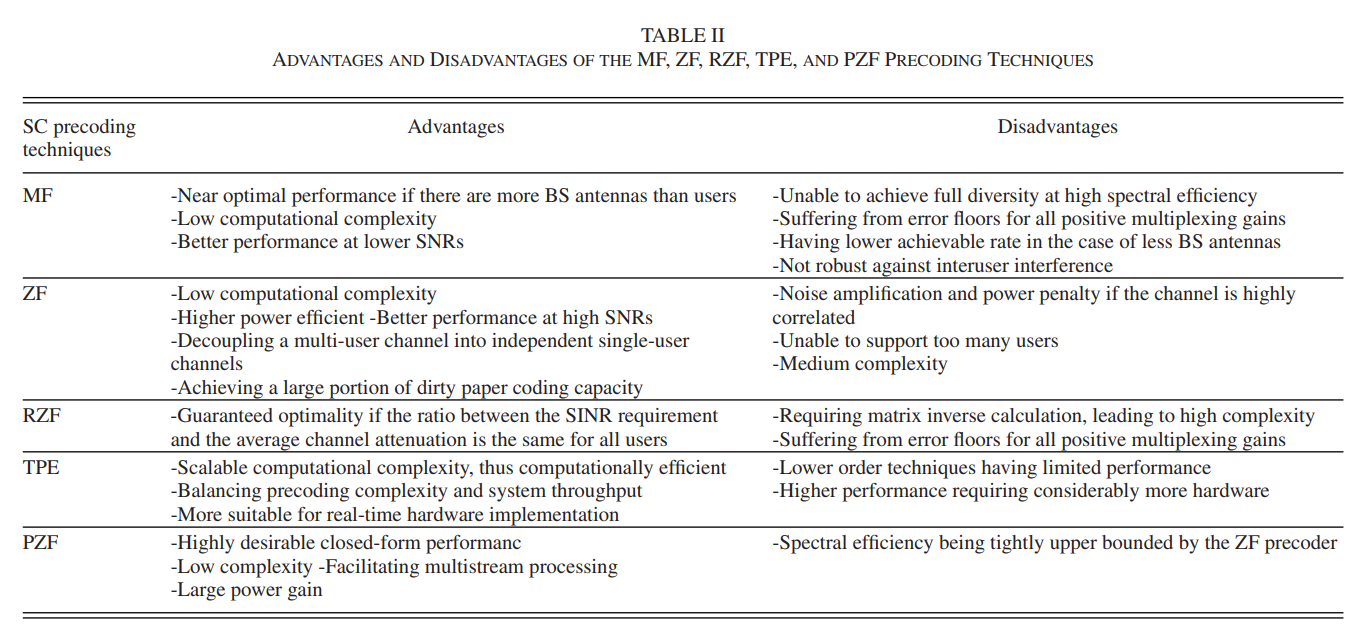
\includegraphics[width=0.99\textwidth]{线性precoder优缺点对比.PNG}
    \caption{优缺点对比}
    \label{kjdfgshafgdad}
\end{figure}

\subsection{基于AI的预编码算法}
\begin{enumerate}
    \item \emph{Kyeongbo Kong, Woo-Jin Song, Moonsik Min, Deep-learning-based precoding in multiuser MIMO downlink channels with limited feedback, 2008.0417}\par
        基于深度学习的均衡,反馈和预编码,下行MU-MIMO系统。基站侧发送预编码使用transmitter DNN实现,每个receiver DNN引入二值化层来模仿量化过程,从而使能端到端训练。由于二值化层的引入导致网络的梯度失真从而容易陷入局部极小值,网络训练过程中引入了辅助训练网络作为教导网络,有效避免陷入局部极小值。与传统的线性预编码相比,该网络通过端到端训练达到了更高的和速率。
    \item \emph{Novel MMSE Precoder and Decoder Designs Subject to Per-antenna Power Constraint
    for Uplink Multiuser MIMO Systems, I-Tai Lu, Jialing Li and Enoch Lu, 2009}\par
        关于多用户MIMO上行预编码的文章,理论比较多。文中提到,最经典的点对点MIMO系统在发送总功率一定时,最优预编码矩阵有最优解,但是在每根天线的功率有限或扩展到多用户MIMO,闭式解不存在,对于MU-MIMO,每个用户总功率有限时,可以通过两种方法寻找数值解,TCIO和GIA。
    \item \emph{Evolution of Uplink MIMO for LTE-Advanced}\par
        LTE中上行MIMO的技术介绍
    \item \emph{Deep Learning based Hybrid Precoding for mmWave Massive MIMO system using ComcepNet, 2020.7}\par
        提出了新的预编码网络结构”ComcepNet“,该网络结合了复数卷积块和 Inception 网络的特征,展现了比autoprecoder更好的性能。
    \item \emph{Deep Learning Based Precoder Design in MIMO Systems with Finite-Alphabet Inputs,2020}\par 
        有限元预编码
    \item \emph{Deep Learning for Distributed Channel Feedback and Multiuser Precoding in FDD Massive MIMO, 20.07}\par
        多用户信道估计和反馈问题可以视为一个分布式信源编码问题。与传统的每个用户独立估计信道信息不同,文章提出联合设计导频并且接收端使用DNN直接将接收导频映射为反馈bit,然后基站将所有用户的反馈bit直接映射为预编码矩阵,可以显著低提高整机性能。文章进一步提出鲁棒化设计策略,并且泛化DNN结构使之适应可变用户和可变的反馈bit。Numerical results show that the DNN-based approach with short pilot sequences and very limited feedback overhead can already approach the performance of conventional linear precoding schemes with full CSI.
    \item \emph{Deep Unfolding for Communications Systems: A Survey and Some New Directions,2019}\par 
        本文综述了深度展开的原理,并讨论了其在通信系统中的最新应用,重点讨论了多天线(MIMO)无线系统中的检测和预编码以及纠错码的信念传播译码。
    \item \emph{Deep reinforcement learning approach to MIMO precoding problem: Optimality and Robustness, 2020}\par 
        强化学习
    \item \emph{Model-Driven Deep Learning for Massive Multiuser MIMO Constant Envelope Precoding} \par 
        常包络预编码设计可以显著降低硬件损耗和功率损耗,但是已有的常包络预编码算法计算复杂度高。文章提出使用模型驱动的方式将深度学习与conjugate gradient algorithm结合,原始迭代算法展开并添加可训练参数,通过数据学习有效的参数。仿真结果表明该网络能有效抑制多用户干扰和计算复杂度。
    \item \emph{}
    
\end{enumerate}

% \part{LAtex语法学习}
\section{Latex语法学习}
\subsection{伪代码}
\href{伪代码}{http://hustsxh.is-programmer.com/posts/38801.html}
\paragraph{algorithmic和algorithmics}
algorithmic和algorithmicx,这两个包很像,很多命令都是一样的,只是algorithmic的命令都是大写,algorithmicx的命令都是首字母大写,其他小写(EndFor两个大写)。下面是algorithmic的基本命令
还有algorithm2e,latex的与algorithm相关的包常用的有几个,algorithm、algorithmic、algorithmicx、algorithm2e,可以大致分成三类,或者说三个排版环境。最原始的是使用algorithm+algorithmic,这个最早出现,也是最难用的,需要自己定义一些指令。第二个排版环境是algorithm+algorithmicx,algorithmicx提供了一些宏定义和一些预定义好了的环境(layout),指令类似algorithmic。第三个是algorithm2e,只需要一个包,使用起来和编程的感觉很像,也是我更倾向使用的包。下面是使用algorithm2e的例子。[1]
\subsection{超链接}
需要的宏包 hyperref, 

\subsection{插入图片}

\subsection{tikz绘图}
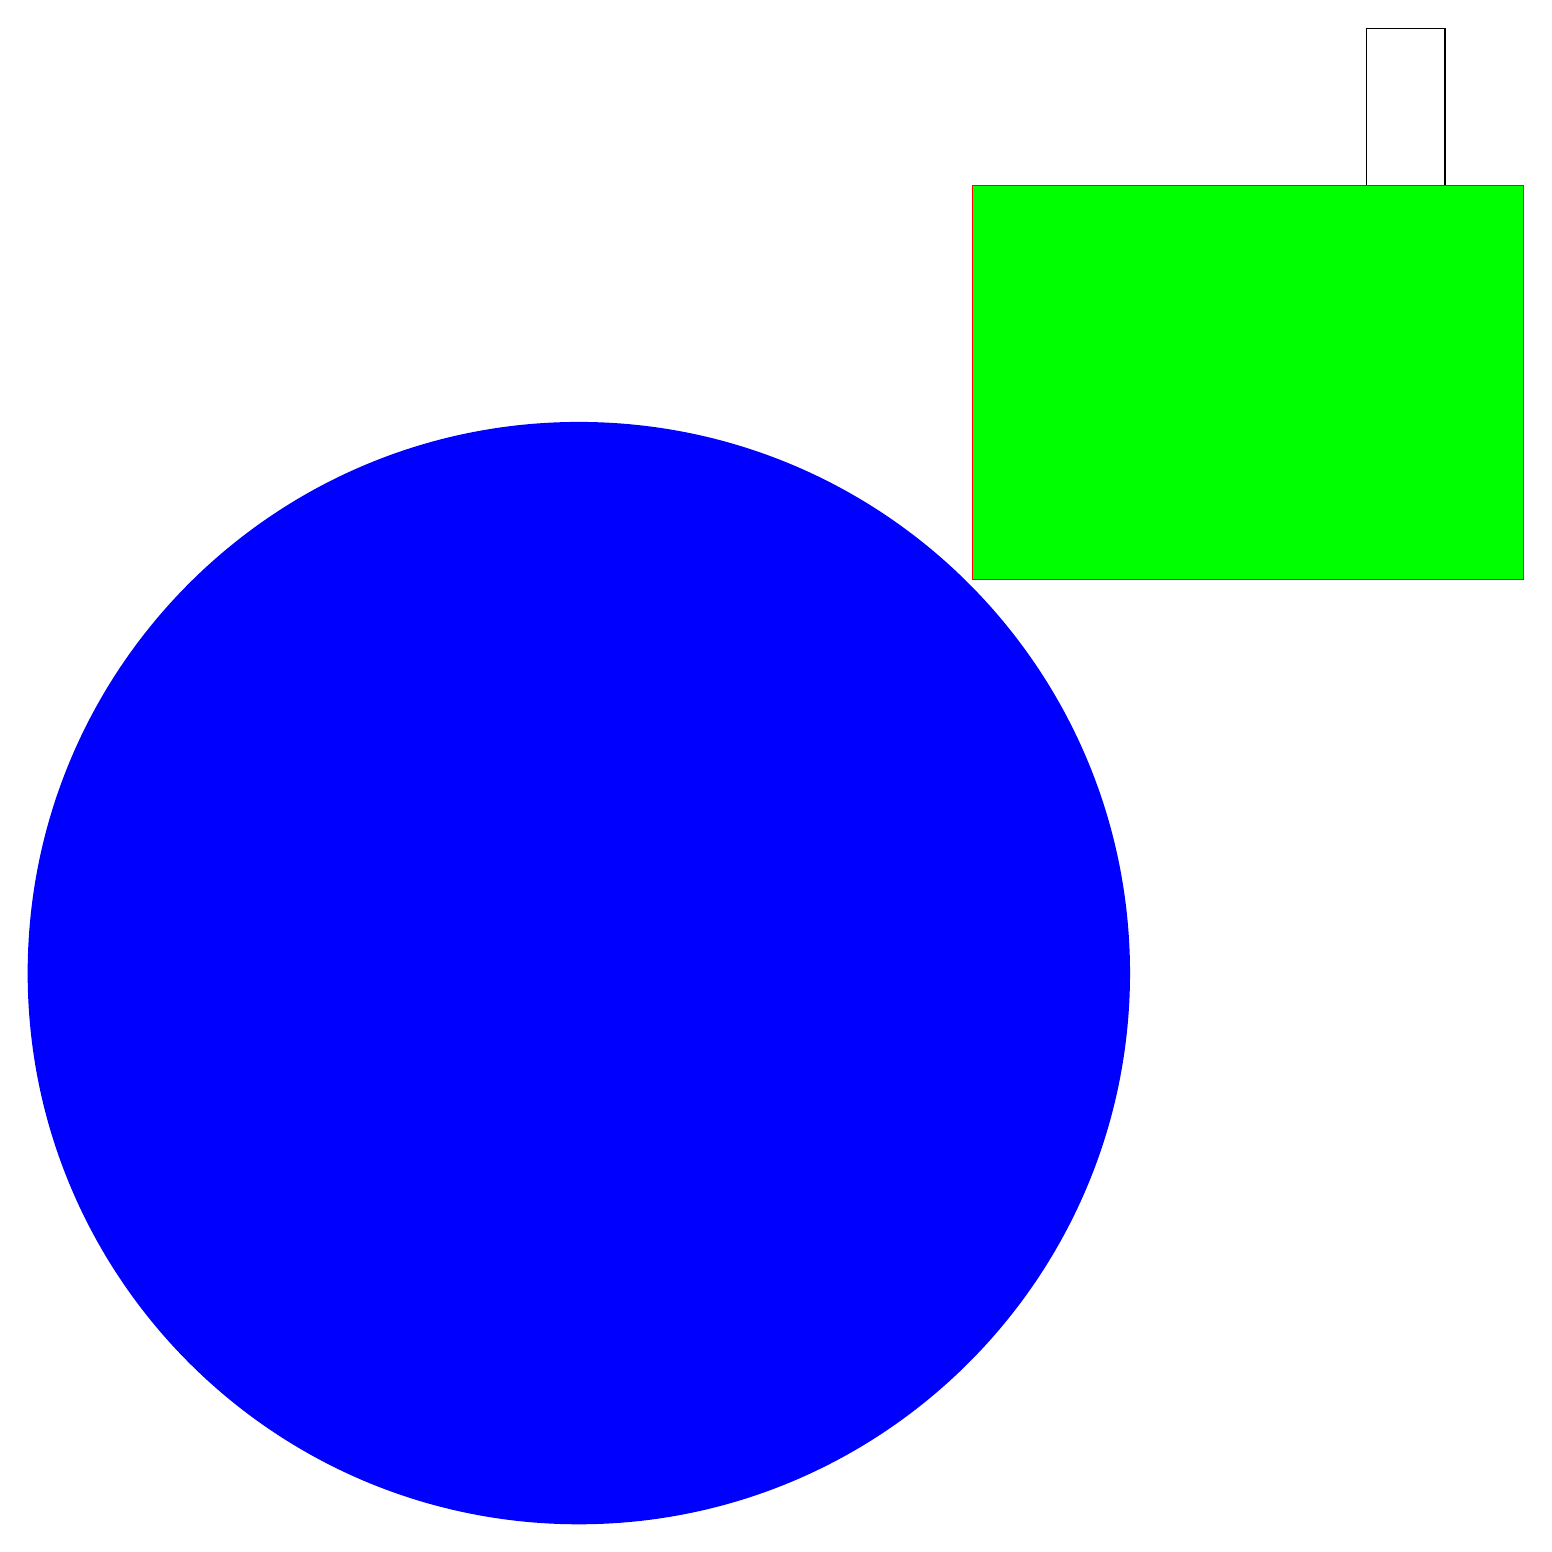
\begin{tikzpicture}
    \draw[red, -latex](0,0)--(5,5);
    \draw (5,5) rectangle (6,7);
    \filldraw[draw=red, fill=green] (0,0) rectangle (7,5);
    \fill[blue](-5,-5) circle [radius=7];
\end{tikzpicture}
% \mint{python}|test.py|		% 这里以Python语言为例。双竖线中是文件名
% \begin{minted}[mathescape,	% 中括号中的内容用于控制代码显示的格式,可以依照喜好修改
%                linenos,
%                numbersep=5pt,
%                gobble=2,
%                frame=lines,
%                framesep=2mm]{python}
% 	...		% 此处插入代码块,需要缩进
% \end{minted}
\tikzset{myarroe/.style={blue, thick,->}}
\begin{tikzpicture}
    \draw[myarroe] (0,0)--(5,5);
\end{tikzpicture}
\newpage
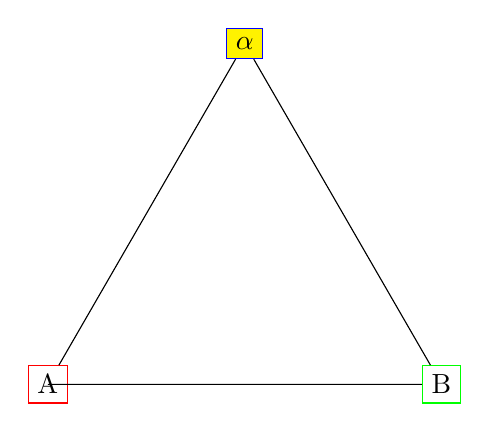
\begin{tikzpicture}
    \node[draw=red] (A) at (0,0) {A};
    \node[draw=green] (B) at (5,0) {B};
    \node[draw=blue,fill=yellow] (C) at (60:5) {$\alpha$};
    \filldraw (A.center) -- (B) -- (C) -- (A);
\end{tikzpicture}

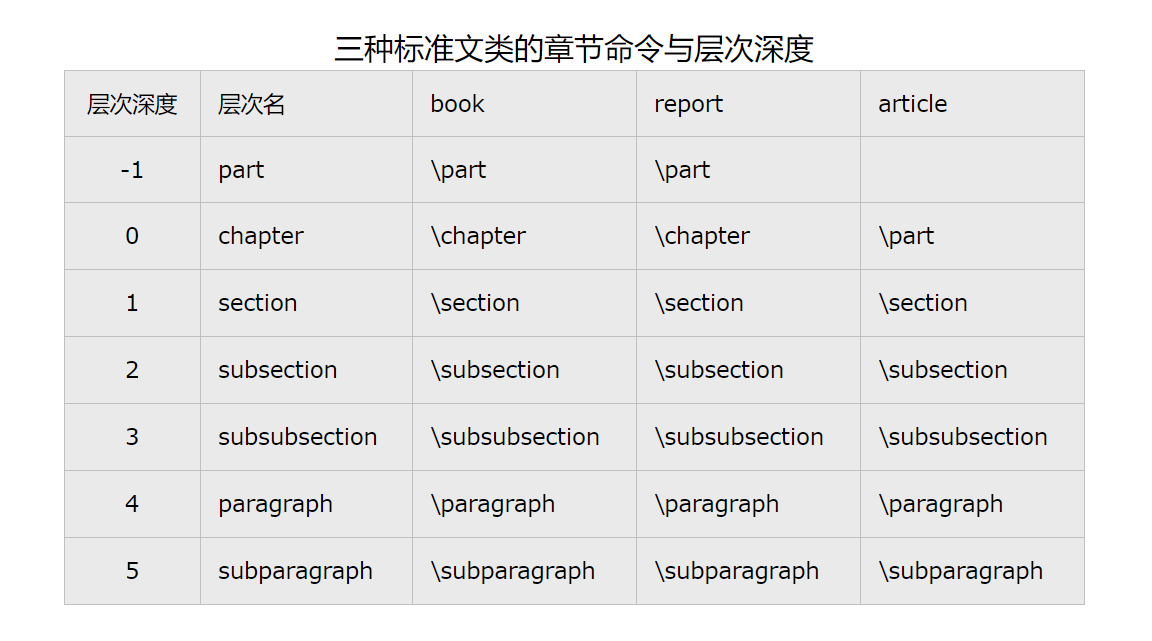
\includegraphics[width=\textwidth]{latex文档层次.PNG}



\begin{tikzpicture}
    \draw (0,0) node[left]{$A$} -- node[left]{$c$} (1,3)node[above] {$B$} --node[right]{$a$} (3,0) node[right]{$C$} -- node[below]{$b$}(0,0);
\end{tikzpicture}

\begin{lstlisting}[language={java}]
public class Main {
    public static void main(String[] args)
    {
        System.out.println("Hello,World");
    }
}
\end{lstlisting}
\section{Latex字体}
\subsection{Latex字母的三种类体}
正体 $\rm{R}$
\begin{lstlisting}
    $\rm{R}$
\end{lstlisting}
花体1 $\mathcal{R}$
\begin{lstlisting}
    $\mathcal{R}$
\end{lstlisting}
花体2 $\mathbb{R}$
\begin{lstlisting}
    $\mathbb{R}$
\end{lstlisting}
花体3 $\mathscr{R}$
\begin{lstlisting}
    $\mathscr{R}$
\end{lstlisting}
dd 
\bibliographystyle{plain}      % 设置引用格式的风格
\bibliography{reference.bib}   % 引用自己的bib文件,保证在当前文件的目录下
\end{document}